\begin{figure}
	\centering
	
	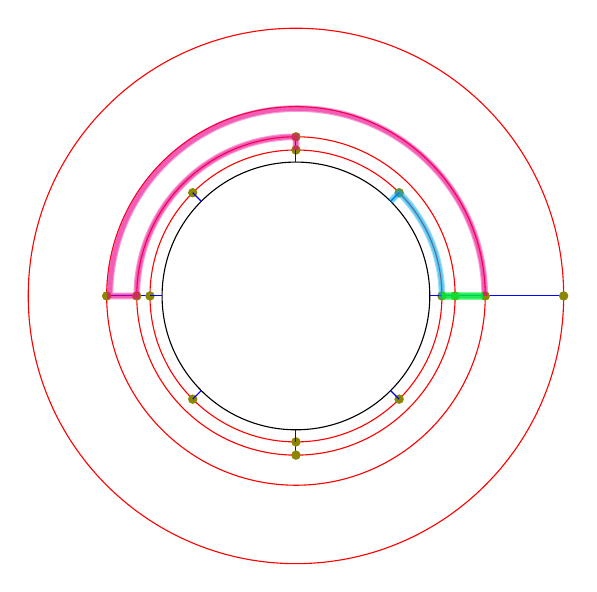
\begin{tikzpicture}[scale=1.7]
		
		
		\draw (0,0) circle (1);
		\draw[red] (0,0) circle (2);
		\draw[red] (0,0) circle (2^0.5);
		\draw[red] (0,0) circle (2^0.25);
		\draw[red] (0,0) circle (2^0.125);
		
		
		\draw[blue] (2,0);
		
		\draw[blue] (2,0) --  (1,0);	
		\draw[blue] (-2^0.5,0) -- (-1,0);	
		\draw[blue] (0, 2^0.25) -- (0,1);	
		\draw[blue] (0, -2^0.25) -- (0,-1);	
		
		\fill[olive] (2,0) circle (1pt);
		\fill[olive] (2^0.5,0) circle (1pt);
		\fill[olive] (-2^0.5,0) circle (1pt);
		
		\foreach \angle in {0,90,180,270}
		\fill[olive] (\angle:2^0.25) circle (1pt);
		
		\foreach \angle in {0,45,90,135,180,225,270,315}
		\fill[olive] (\angle:2^0.125) circle (1pt);
		\foreach \angle in {0,45,90,135,180,225,270,315} 		
		\draw[blue] (\angle:2^0.125) -- (\angle:1);
		
		

\draw [magenta,-,
double=magenta,
double distance=4\pgflinewidth, opacity=0.4,
] (1.41,0) arc (0:180:1.4) -- (-1.189,0) arc (180:90:1.189) -- (0,1.0905);

\draw [cyan,-,
double=cyan,
double distance=4\pgflinewidth, opacity=0.4,
] (1.4,0) -- (1.0905,0) arc (0:45:1.0905) -- (45:1) ;


\draw [green,-,
double=green,
double distance=6\pgflinewidth, opacity=0.4,
] (1.0905,0) -- (1.4,0);


\draw[blue] (2,0);

		
	\end{tikzpicture}
	
	\caption{The three parts of an itinerary $\eta$. The green path is  $\gamma _{m,n}$,  the cyan and magenta are $\gamma _m$ and $\gamma_n$.
	} \label{fig:Three-parts-of-eta}
\end{figure}

